\documentclass[12pt, a4paper]{article}
\usepackage{setspace}
\usepackage[centertags,reqno]{amsmath}
\usepackage{amssymb}
\usepackage{graphics,subfigure}
\usepackage[dvips]{graphicx}
\usepackage[dvipsnames]{xcolor}
\usepackage[hidelinks]{hyperref}
\usepackage{appendix}
\usepackage{natbib}
\usepackage{pdflscape}
\usepackage[showframe=false]{geometry}
\usepackage{mdframed}
\usepackage{eurosym}
%\usepackage{textcomp}
\usepackage{multirow}
\usepackage{caption}
\usepackage{hyphenat}
\usepackage{tikz}
\newcommand{\mybox}[2]{{\color{#1}\fbox{\normalcolor#2}}}

\usepackage{tabularx,calc}
\usepackage{dcolumn}                    % Aligns tables on the decimal point
\newcolumntype{d}[1]{D{.}{.}{#1}}       %       Aligns on dot
\newcolumntype{.}{D{.}{.}{3.5}}         %       Somehow it works better
\newcolumntype{C}{@{\extracolsep{.6cm}}c@{\extracolsep{0pt}}}
\usepackage{threeparttable}
\usepackage{siunitx,booktabs}
\sisetup{
    detect-all,
    round-integer-to-decimal = true,
    group-digits             = true,
    group-minimum-digits     = 4,
    group-separator          = {\,},
    table-align-text-pre     = false,
    table-align-text-post    = false,
    input-signs              = + -,
    input-symbols            = {*},
    input-open-uncertainty   = ,
    input-close-uncertainty  = ,
    retain-explicit-plus
}

\begin{document}

\section{Research question + design}

In this paper, we use an online experiment to study whether the distribution of risks one faces influences their willingness to take risks.
Participants can earn either a high or a low payoff by accepting a lottery, or a safe intermediary payoff by rejecting the lottery.
We use a Becker--Degroot--Marschak mechanism and ask them for their minimum acceptable probability ($MAP$) of the lottery's high payoff, $p$, for preferring the lottery over the safe payoff.

Participants make decisions in three different treatments.
They state their $MAP$ when $p$ comes from a uniform distribution, a left-skewed distribution and a right-skewed distribution.
We call the corresponding treatments `the Uniform', `the Good' and `the Bad'.
%When making their decision, participants see a graphical representation of a distribution over lotteries with two possible outcomes (high and low), but varying probabilities for each outcome.
After they report their three $MAP$s, a distribution is drawn and a lottery is drawn at random from that distribution to determine their payoff.
Depending on how $p$ in this lottery compares to $MAP$, their payoff is either the outcome of the lottery or the safe payoff.
By construction, in some treatments it is more likely that a lottery with a high chance of a high payoff is drawn.
%We use three distributions over lotteries.
%The distributions are ordered in terms of the expected payoff over the entire distribution, as their name suggests: the Good, the Bad, and the Uniform (the Good $>$ the Uniform $>$ the Bad).

We present lotteries graphically via 32 wheels of fortune with 15 sectors each.
Dark blue sectors symbolize the high payoff (\pounds4), light blue sectors---the low payoff (\pounds1).
The sure payoff is \pounds2.
In each treatment, participants see the wheels sorted in ascending order by the probability of the favorable outcome $p$, with the 32 wheels equally distributed over four rows.

\begin{figure}[h!]
  \centering
 {\includegraphics[width=\linewidth]{Fig1_Left_15.pdf}}
  \caption{The Good distribution}
  \label{fig:TheGood}
\end{figure}

Figure \ref{fig:TheGood} shows the distribution of lotteries for the Good treatment.
The number in each wheel is the number of sectors yielding a high payoff (ranging from 0 to 15).
The Uniform distribution has equal chances of occurrence for each of the possible wheels.
The Bad distribution has an overall chance of a high payoff equal to 0.2895.
The distribution in Good mirrors the one in Bad: its overall expected chance of a high payoff is one minus that in Bad (0.7105), it has the same variance and minus the skewness of the Bad distribution.
Table \ref{tab:distr} presents the distributions.


\begin{table}[htbp]
\centering \caption{The treatments: the distribution of chances of a high payoff $p$}\label{tab:distr}
\begin{threeparttable}
\begin{tabular}
   {@{}
	*5c
	@{}
	}
\toprule
	&	\multicolumn{3}{c}{\# of wheels}&\\
	\cmidrule{2-4}
\# of high payoff sectors 	&	{The Good}&{The Bad}&	{The Uniform}& {Probability of high payoff $p$}\\
\midrule
0	    &	1&       8&	2& 0   \\
1	    &	1&       4&	2& 0.07\\
2	    &	1&       4&	2& 0.13\\
3	    &	1&       3&	2& 0.20\\
4	    &	1&       2&	2& 0.27\\
5	    &	1&       1&	2& 0.33\\
6	    &	1&       1&	2& 0.38\\
7	    &	1&       1&	2& 0.47\\
8	    &	1&       1&	2& 0.53\\
9	    &	1&       1&	2& 0.60\\
10	    & 1&       1&	2& 0.67\\
11	    & 2&       1&	2& 0.73\\
12	    &	3&       1&	2& 0.80\\
13	    &	4&       1&	2& 0.87\\
14	    &	4&       1&	2& 0.93\\
15	    &	8&       1&	2& 1   \\
\midrule
Total \# of wheels	&	32&       32&	32&\\
\bottomrule

\end{tabular}
\end{threeparttable}
\end{table}

Participants are told that one of the wheels will be drawn at random, with all wheels having an equal chance to be drawn.
They are asked to state a \textit{minimum acceptable frequency}: the lowest number of dark blue sectors in the randomly drawn wheel such that they prefer to spin the wheel instead of receiving the sure payoff.\footnote{
We decided to use frequencies instead of probabilities because there is evidence that participants have an easier time expressing choice this way \citep{Quercia2016}.}
Specifically, they have to answer: ``Which wheels would you like to spin for your bonus?'' by inserting an integer between 0 and 15 in the blank space: ``I prefer to spin wheels which have at least \rule{1cm}{0.15mm} dark blue sectors.''\footnote{
We chose the setup with wheels of fortune as we wanted to make the task easy to understand.
Despite our approach being discrete, we interpret the frequencies ($x$ out of 15) as minimum acceptable probabilities.
}

%We use a within-subject design.
%One of the three decisions participants make (the three $MAPs$) is relevant for payment.

\section{Short summary of results}

We find that $$MAP^*_{Good} > MAP^*_{Uni} > MAP^*_{Bad}$$
This is true for between-individual comparisons.
The differences are highly significant.
Figure \ref{fig:MeanMAPs} shows that this is true for all treatment sequences.
When looking at within-individual comparisons, 44\% report the same $MAP$ in all treatments, while for 42\% at least one of the inequalities holds (for 38\%, two of the three $MAPs$ are tied, while the third one follows the same ordering as for the between-individuals comparison e.g. $$MAP^*_{Good} > MAP^*_{Uni} = MAP^*_{Bad}$$

\begin{figure}[h!]
	\centering
	{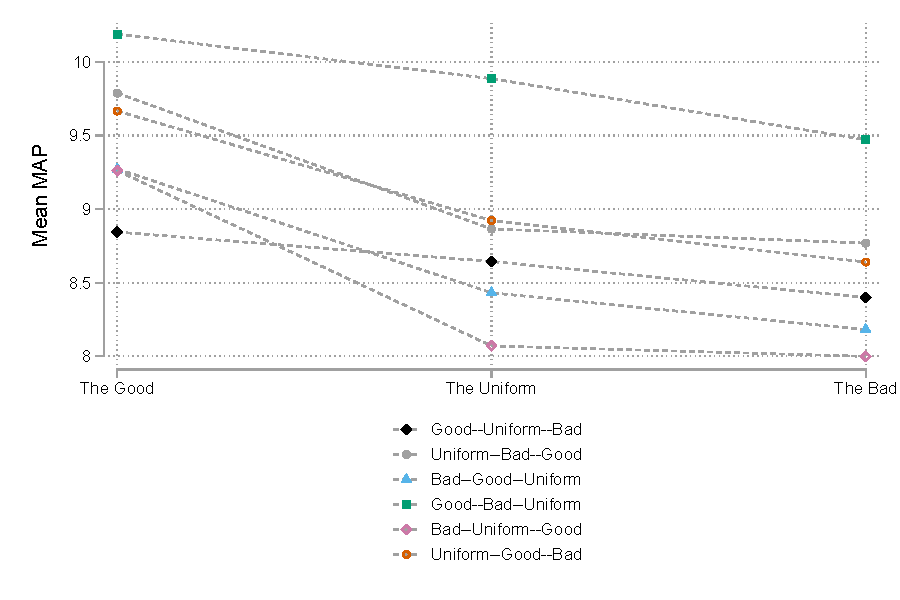
\includegraphics[width=\linewidth]{Fig2_MeanMAPs_nice.pdf}}
	\caption{Mean $MAPs$ by treatment and decision sequence}
	\label{fig:MeanMAPs}
\end{figure}

\section{Predictions according to KR}

Referees suggested we use a reference-dependent model to check whether it could explain our findings.
We modeled utility following \cite{Koszegi2007} (KR): $$u(w|r)=m(w)+\mu(m(w)-m(r))$$
where $w$ is the outcome (which could be low, safe or high), $m(.)$ is consumption utility, $r$ is the referent and $\mu(m(w)-m(r))$ is gain-loss utility.
We made the following simplifying assumptions: $m(w)=w$, loss aversion is two-to-one and $r$ is the distribution of lotteries in each treatment (the exogenous part) including one's own $MAP$ (the endogenous part).
The intuition behind this choice of referent is that participants are correct about what they get in expectation for a certain $MAP$.

In the accompanying Mathematica file, we calculate and plot expected utility in all three treatments as a function of $MAP$.
This is a tedious (but straightforward) calculation because of the complexity of the referent.
We find that KR with the above assumptions predicts the opposite ordering to the one we find: $$MAP^*_{Good} < MAP^*_{Uni} < MAP^*_{Bad}$$

There are two possible options:
\begin{enumerate}
 \item We made a mistake, either in our assumptions or in our calculation.
 \item KR is not applicable in our setting.
\end{enumerate}
Option 2 is more intriguing, but begs the question: why?\footnote{
We considered taking $r$ as only the distribution.
This doesn't have an intuitive appeal: it reflects choosing a $MAP$ of zero.
In this case, KR predicts $MAP^*$ to be the same in all treatments.
}

\clearpage
\pagebreak
\bibliographystyle{apalike}
\bibliography{MAPs}
\end{document}
